%%%%%%%%%%%%%%%%%%%%%%%%%%%%%%%%%%%%%%%%%
% a0poster Portrait Poster
% LaTeX Template
% Version 1.0 (22/06/13)
%
% The a0poster class was created by:
% Gerlinde Kettl and Matthias Weiser (tex@kettl.de)
% 
% This template has been downloaded from:
% http://www.LaTeXTemplates.com
%
% License:
% CC BY-NC-SA 3.0 (http://creativecommons.org/licenses/by-nc-sa/3.0/)
%
%%%%%%%%%%%%%%%%%%%%%%%%%%%%%%%%%%%%%%%%%

%-----------------------------------------------------------------------------
%	PACKAGES AND OTHER DOCUMENT CONFIGURATIONS
%-----------------------------------------------------------------------------

\documentclass[a0,portrait]{a0poster}

%% % sans-serif config:


\usepackage[english]{babel}
\usepackage[utf8]{inputenc}
\usepackage[T1]{fontenc}
\renewcommand{\familydefault}{\sfdefault}

\usepackage{multicol} % This is so we can have multiple columns of
                      % text side-by-side
\columnsep=100pt % This is the amount of white space between the
                 % columns in the poster
\columnseprule=3pt % This is the thickness of the black line between
                   % the columns in the poster

\usepackage[svgnames]{xcolor} % Specify colors by their 'svgnames',
                              % for a full list of all colors
                              % available see here:
                              % http://www.latextemplates.com/svgnames-colors

\usepackage{tgheros}


%% \usepackage{times} % Use the times font
%% \usepackage{palatino} % Uncomment to use the Palatino fon

\usepackage{graphicx} % Required for including images
\graphicspath{{figures/}} % Location of the graphics files
\usepackage{booktabs} % Top and bottom rules for table
\usepackage[font=small,labelfont=bf]{caption} % Required for
                                              % specifying captions to
                                              % tables and figures
\usepackage{amsfonts, amsmath, amsthm, amssymb} % For math fonts,
                                                % symbols and
                                                % environments
\usepackage{wrapfig} % Allows wrapping text around tables and figures

%\usepackage{sfmath}
\usepackage{sansmath} %additional math
\sansmath

\usepackage{mathsetup}

\usepackage{bibconfig}

\usepackage{titlesec}

\titlespacing*{\section}
{0pt}{2.5ex plus 1ex minus .2ex}{1.5ex plus .2ex}


\makeatletter
\g@addto@macro\normalsize{%
  \setlength\abovedisplayskip{18pt}
  \setlength\belowdisplayskip{18pt}
  \setlength\abovedisplayshortskip{16pt}
  \setlength\belowdisplayshortskip{16pt}
}
\makeatother


\addtolength{\parskip}{0.5\baselineskip}
\parindent 0pt

\definecolor{gblue}{RGB}{27,98,183}

\begin{document}

%-----------------------------------------------------------------------------
%	POSTER HEADER 
%-----------------------------------------------------------------------------

% The header is divided into two boxes:
% The first is 75% wide and houses the title, subtitle, names, university/organization and contact information
% The second is 25% wide and houses a logo for your university/organization or a photo of you
% The widths of these boxes can be easily edited to accommodate your content as you see fit
\vspace{-5cm}

%\fbox{
\begin{minipage}[b]{0.75\linewidth}
  \veryHuge \textbf{Models of } \color{Black}\\[1.5cm] 
%\Huge\textit{}\\[2cm] % Subtitle
  \huge \textbf{Felix Z. Hoffmann$^{1,2}$, Jochen Triesch$^1$}\\[0.5cm] % Author(s)
\large $\quad ^1$Frankfurt Institute for Advanced Studies (FIAS), Johann Wolfgang Goethe University, Frankfurt am Main, Germany\\[0.2cm] % University/organization
$\quad ^2$International Max Planck Research School for Neural Circuits, Max Planck Institute for Brain Research, Frankfurt am Main, Germany\\[0.4cm]
\Large \texttt{hoffmann@fias.uni-frankfurt.de}\\
\end{minipage}
%}
%
%\fbox{
\begin{minipage}[b]{0.25\linewidth}
  \centering
  
  
\includegraphics[width=10cm]{goethe-logo.pdf}\\
  \vspace{2.8cm}
  
\includegraphics[width=12.5cm]{FIAS-logo.pdf}\\
  \vspace{2cm}
  
\end{minipage}
%}
%\vspace{0.2cm} % A bit of extra whitespace between the header and poster content

%-----------------------------------------------------------------------------

\begin{multicols}{2} % This is how many columns your poster will be
                     % broken into, a portrait poster is generally
                     % split into 2 columns

  \columnbreak
\section*{\LARGE Log-normal distributions of synaptic weights in noise driven networks}

In cortical circuits the distribution of synaptic weights has been repeatedly reported to be a log-normal \cite{Song2005}. in which very few strong weights are embedded in a sea of small weights. A number of computational models address the . Typically the result . Here we are following a hypothesis that not much is needed.


\section*{Network model}

The network is thus completely noise driven and devoid of correlations.



\section*{Results}

\begin{center}\vspace{1cm}
  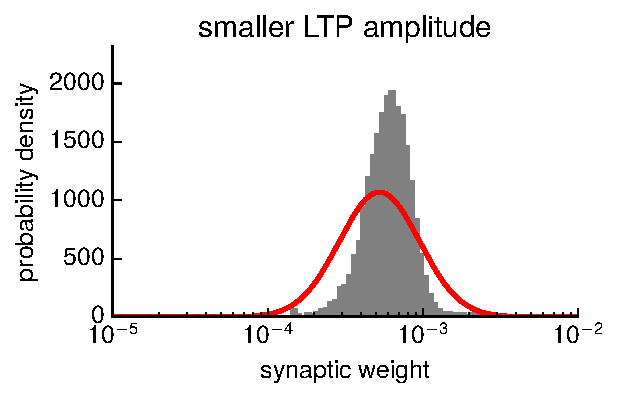
\includegraphics[width=.49\columnwidth]{%
    figures/syn_lnt_gnw_e07036_16.pdf}
  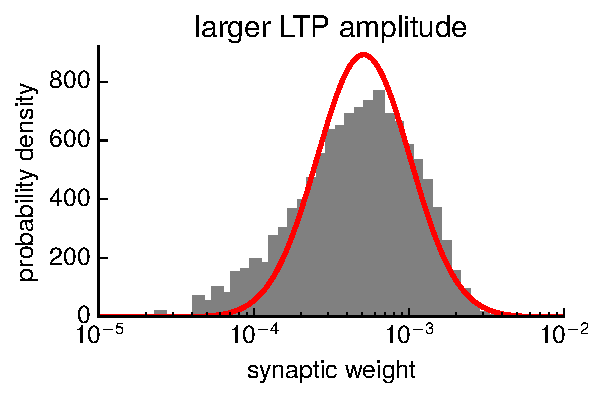
\includegraphics[width=.49\columnwidth]{%
    figures/syn_lnt_gnw_e07036_17.pdf}

  \captionof{figure}{}
\end{center}\vspace{1cm}


\begin{center}\vspace{1cm}
  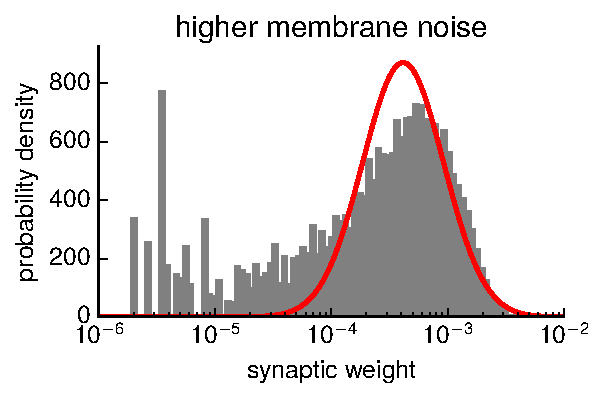
\includegraphics[width=.49\columnwidth]{%
    figures/syn_lnt_gnw_b20efe_0_highmem.pdf}
  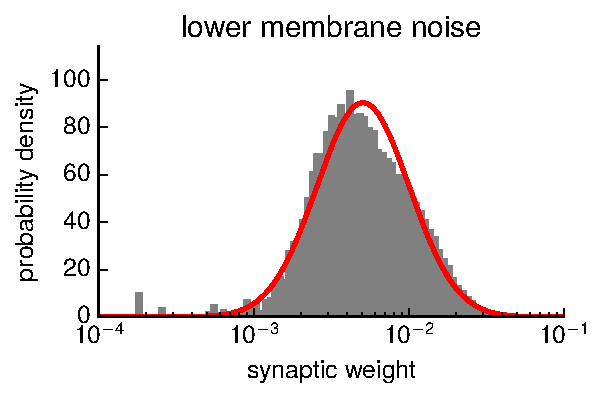
\includegraphics[width=.49\columnwidth]{%
    figures/syn_lnt_gnw_b20efe_0_lowmem.pdf}

  \captionof{figure}{$T=\text{\SI{900}{s}}$, LTD=-0.1 LTP}
\end{center}\vspace{1cm}


\section*{Coupled Networks}


  \columnbreak
\section*{\LARGE Modelling synaptic lifetime distributions with Kesten processes}

In an experimental study by \textcite{Loewenstein2015} chronic in-vivo two-photon imaging suggested that the lifetime dynamics of spines in the neocortex follow a power law. Motivated by results from detailed network simulations, we here consider a simple stochastic model based on the Kesten process in order to analyze how different properties of a cortical network might affect the lifetime distributions of synaptic spines.

\vspace{-0.4cm}
\section*{Model}

Kesten processes have been used before \cite{Statman2014} to describe spine size dynamics. In this model, a given spine size $X_n$ at time step $n$ is updated as
%
\begin{align}
  X_{n+1} = a_n X_n + b_n. \label{eq:kesten}
\end{align}
%
In this further simplified form we take $a_n$ to be a fixed value of $a_n < 1$, while the additive change is in each time step drawn from a normal distribution, $b_n \sim \mathcal{N}(\mu_b, \sigma_b^2)$. Then, to model synapse growth and pruning processes, we consider a population of $N$ synapses. Each synapse has a random time $T_{\mathrm{init}}$, uniformly distributed in $[0,T_{\text{max}}]$, at which it is initialized with size $X_0$. The synapse size $X_t$ then evolves according to \eqref{eq:kesten}.

\medskip

The lifetime of the synapse is the number of time steps from $T_{\text{init}}$ until for the first time $X_t < X_{\mathrm{prune}}$. In this case the synapse gets pruned and a new synapse with size $X_0$ is inserted in the network (Fig.~\ref{fig:km}). In the case that $X_t$ doesn't fall below $X_{\mathrm{prune}}$ until $T_{\text{max}}$, the lifetime is recorded as $T=T_{\text{max}}-T_{\text{init}}$. At the end of the simulation the sizes $X_{T_{\text{max}}}$ are recorded for all $N$ synapses.

\begin{center}\vspace{1cm}
  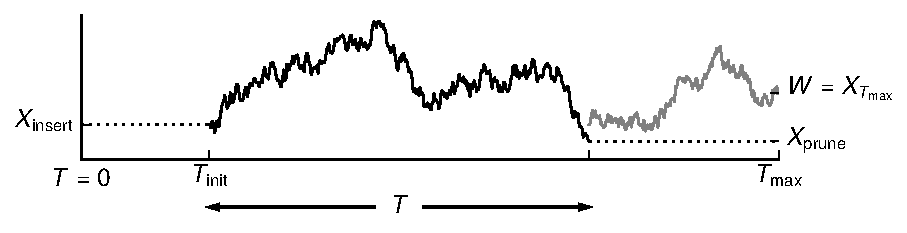
\includegraphics[width=0.85\columnwidth]{%
    figures/abstract_fig.pdf}
  %% /home/fh/sci/lab/syn_lt/kesten_model/note_x/km_ca_rts_dd/img/abstract_fig.png}
  \captionof{figure}{Adapted Kesten simulation model allows the tracking of lifetimes and size distributions}
  \label{fig:km}
\end{center}\vspace{1cm}


\section*{Results}

We simulated \SI{5e5} synapses evolving as Kesten processes and recorded lifetime and weight distributions. For unbiased additive change ($\mu_b =0$), a power law like distribution of synaptic lifetimes emerges (Fig.~\ref{fig:lifetimes}A). The distribution of spine sizes $X_{T_{\text{max}}}$ resembles a log-normal distribution, as one might expect from findings on the synaptic weight distributions in cortical circuits \cite{Song2005}.

\vspace{1.2cm}
\begin{overpic}[width=\columnwidth]%
  % 110, 133
  {figures/lifetimes_weights.pdf}
  %\put(32,\ylin){anisotropic}
  \put(1,28){\normalfont \textbf{A}}
  \put(52,28){\normalfont \textbf{B}}
\end{overpic}
\captionof{figure}[format=hang,indention=1cm]{Dynamical properties of network connectivity modelled by Kesten processes. \textbf{A} Lifetime distribution of synapses created at time step $T_{\text{init}}$ uniformly distributed in $[0, T_{\text{max}}]$. \textbf{B} Distribution of spine sizes $X_{T_{\text{max}}}$ at time step $X_{T_{\text{max}}}$ (grey) and log-normal fit (red). Parameters for both: $a=0.9987$, $\mu_b=0$, $\sigma_b^2=0.22$, $X_{\text{insert}}=0.1$, $X_{\text{prune}}=0.01$. \label{fig:lifetimes}}

\vspace{3cm}

%% \begin{center}\vspace{1cm}
%%   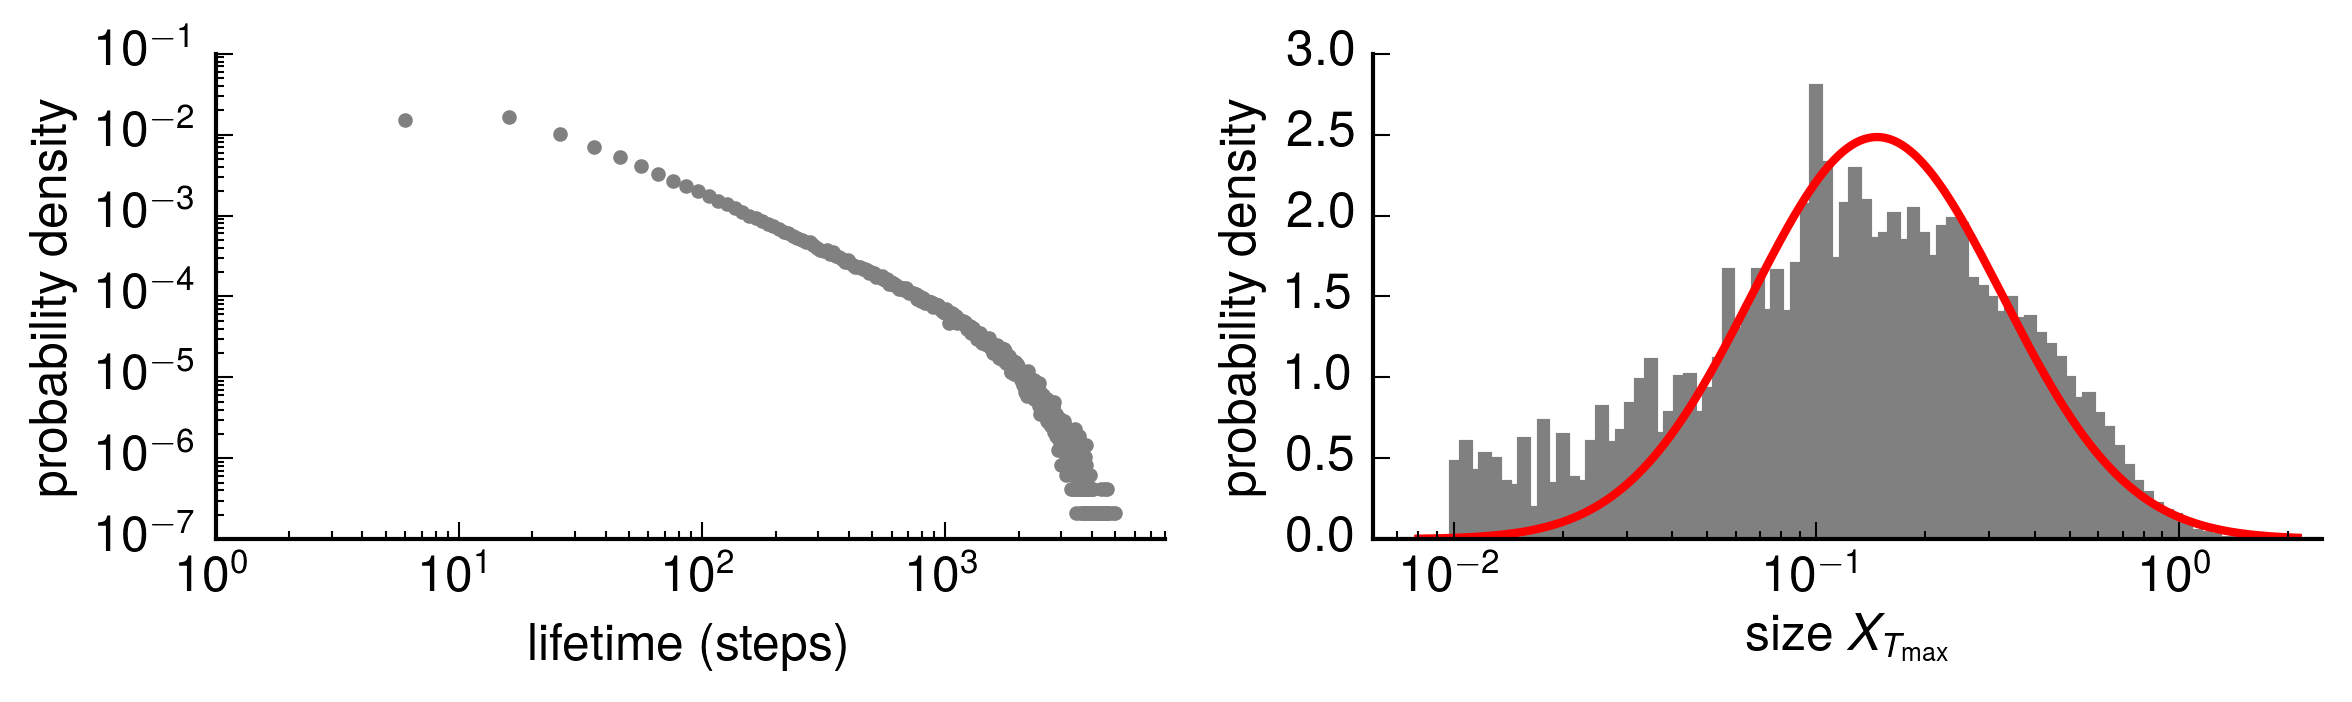
\includegraphics[width=\columnwidth]{%
%%     %% /home/fh/sci/lab/syn_lt/kesten_model/note_x/km_ca_rts_dd/img/lifetimes_weights.png}
%%     figures/lifetimes_weights.png}

%%   \captionof{figure}{}
%%   \label{fig:lifetimes}
%% \end{center}\vspace{1cm}

Next, we explored how different parameters in the model affect the lifetime and spine size distributions. We found that varying $\sigma_b^2$ has little effect on the distributions. Interestingly however, the bias in the additive change affects both distributions significantly. As one might expect, a bias towards increases in size moves the tail of the lifetime distribution towards higher lifetimes (Fig.~\ref{fig:lifemub}A) while shifting the mean of the spine size towards higher values (Fig.~\ref{fig:lifemub}B). This observation matches qualitatively with preliminary results from detailed network simulations in which a higher bias towards LTP resulted in similarly extended lifetimes.

  \vspace{1.4cm}
\begin{overpic}[width=\columnwidth]%
  % 110, 133
  {figures/lifetimes_weights_mub_compare.pdf}
  %\put(32,\ylin){anisotropic}
  \put(1,28){\normalfont \textbf{A}}
  \put(52,28){\normalfont \textbf{B}}
\end{overpic}
  \captionof{figure}{The bias of additive change in size strongly affects both lifetime and weight distributions. \label{fig:lifemub}}

  \vspace{1.8cm}
  




  
  \printbibliography  

\end{multicols}

%% \begin{columns}
%%   %
%%   \begin{column}{.5\textwidth}
%%     \input{sections/abstract}  
%% \input{sections/introduction}

%%   \end{column}
%%   %
%%   \begin{column}{.5\textwidth}

%%       \input{sections/results}
%%   \end{column}
%% \end{columns}


\end{document}
